\documentclass{article}
\usepackage{amssymb}
\usepackage[utf8]{inputenc}
\usepackage[english]{babel}
\usepackage{amsthm}
\usepackage{enumitem}
\usepackage{amsmath}
\usepackage{mathrsfs}
\usepackage{hyperref}
\usepackage{graphicx}
\usepackage{placeins}
\usepackage[hypcap]{caption}
\usepackage{subcaption}
\usepackage[margin=.5in]{geometry}
\usepackage[export]{adjustbox}
\usepackage{listings}
\usepackage{alltt}

\graphicspath{{./p1/Figures/}}

\title{Project 1 Writeup}
\date{03/02/2016}
\author{Andrea Bajcsy \and Charles Parker}

\begin{document}
	\maketitle
	
	\begin{enumerate}
	
	\item[\textbf{WU1}] The classification accuracy, \verb|Acc|, can be expressed by
	
		\begin{alltt}
			Acc = \(\frac{1}{N} \sum\sb{k=1}\sp{N} \) [ datasets.TennisData.Y(k) == h.predictAll(datasets.TennisData.X)(k) ] \\
			\quad  = mean (datasets.TennisData.Y == h.predictAll(datasets.TennisData.X)) 
		\end{alltt}
	
		\verb|datasets.TennisData.Y ==  h.predictAll(datasets.TennisData.X)| produces an array
		that consists of a 1 at the indices the array agree and a 0 elsewhere. The arrays agree
		only when the test label matches the prediction.
	
		\verb|datasets.TennisData.Y > 0| converts all of the negative labels to 0 and keeps the 
		positive labels at 1. Call this new array \verb|a|. Similarly, 
		\verb|h.predictAll(datasets.TennisData.X) > 0)| converts all of the predicted negative
		labels to 0 and keeps the predicted positive labels at 1. Denote this array as \verb|b|.

		\verb|a == b| produces an array that consists of a 1 at the indices the array agree and 
		a 0 elsewhere. The arrays agree only when the test label matches the prediction since the
		-1 labels have essentially been replaced by a 0 label. Therefore, \verb|a == b| is the same
		array as \\
		\verb|datasets.TennisData.Y == h.predictAll(datasets.TennisData.X)|, 
		and the computations are equivalent.
		
	\item[\textbf{WU2}] Training accuracy tends to decrease because as the the number of
		input data points increases while tree height remains constant, the likelihood of
		misclassifying new data points increases. In other words, the tree is not able to learn
		any new features to separate a more diverse sample space. \\
		
		The test accuracy is not monotonically increasing because the initially small samples of
		data are not sufficient to allow inference to the real data distribution. At a certain
		point during testing, the number of data points allows for a sufficiently accurate
		representation of the real data. In other words, the tree is unable to generalize
		from such a small sample size at first. Then, the sample size reaches a threshhold
		that closely matches the true data distribution. Larger samples closely match the relative
		composition of this threshhold sample size. \\
		
		The jaggedness arises from the inability of a small data sample to sufficiently represent
		the true data distribution compared to a large sample. Some small samples, by chance, may
		accurately represent the real distribution, while others, by chance, do not. For this
		reason, some relatively small samples allow for higher test accuracy while the others
		have a low test accuracy, causing the graph to exhibit erratic behavior for small samples.
	
	\item[\textbf{WU3}] We are guaranteed to see training accuracy monotonically increasing as
		the tree gets deeper because we are considering more features to partition the data. On
		the other hand, we expect that test accuracy will increase and then start to decrease in
		a hill-like fashion due to overfitting. 
	
	\item[\textbf{WU4}] There does not appear to be any evidence of overfitting because the test
		accuracy is increasing as the sample size increases.
		
		All figures appear at the end of the document. The train/test curves for various $K$
		values are shown first in Figure \ref{k_figs}, followed the train/test curves for various
		$\epsilon$ in Figure \ref{eps_figs}.
		
	\item[\textbf{WU5}] The results almost mimic those for random data. In higher dimensions, the
		distances between points is more concentrated in a small range, while in lower dimensions,
		the distances between points is more spread out. The exception here is 2 dimensions. Many
		of the points are very close to each other with respect to only 2 features (in fact, they
		are 0 distance apart). This is not necessarily surprising since the two features chosen
		at random are probably black pixels on most images. 8 dimensions is also more spread out
		than on random data. One possible explanation is that pixels are not distrubted randomly
		throughout the image, rather most non-zero pixels are concentrated towards the center
		of the image. Otherwise, the data behaves as expected.
		
		The histogram corresponding to the pairwise distances in all 784 dimensions is in Figure
		\ref{alldims_fig}, and the subsampled dimension data appears in Figure 
		\ref{subsample_fig}.
		
	\item[\textbf{WU6}] The learning curve for the perceptron with 5 epochs is shown in Figure
		 \ref{lc_percept_fig}. The impact of the number of epochs on train/test accuracy is shown
		 in Figure \ref{epoch_tt_fig}.
	
	\end{enumerate}
	
	\begin{figure} [h!]
		\begin{subfigure} [h!]{.4\textwidth}
		
\includegraphics[scale = .45]{LC_k1.png}
		\end{subfigure}
		\hfill
		\begin{subfigure} [h!]{.4\textwidth}
		
\includegraphics[scale = .45]{LC_k2.png}
		\end{subfigure}
		\\
		\begin{subfigure} [h!]{.4\textwidth}
		
\includegraphics[scale = .45]{LC_k5.png}
		\end{subfigure}
		\hfill
		\begin{subfigure} [h!]{.4\textwidth}
		
\includegraphics[scale = .45]{LC_k10.png}
		\end{subfigure}
		\caption{Learning curves for various $K$ values}
		\label{k_figs}
	\end{figure}
	
	
	\FloatBarrier	

	\begin{figure} [h!]
	\centering
		\begin{subfigure} [h!]{.4\textwidth}
		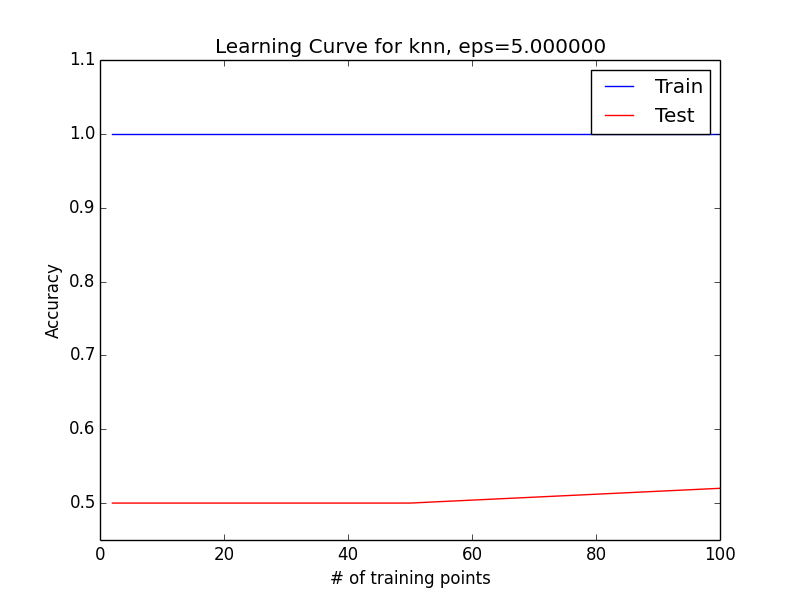
\includegraphics[scale = .45]{LC_eps5_000000.png}
		\end{subfigure}
		\hfill
		\begin{subfigure} [h!]{.4\textwidth}
		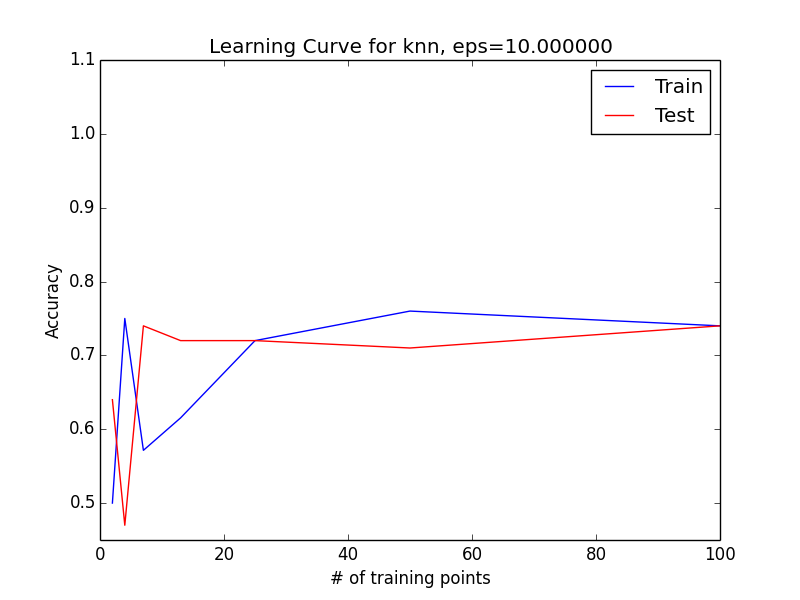
\includegraphics[scale = .45]{LC_eps10_000000.png}
		\end{subfigure}
		\\
		\begin{subfigure} [h!]{.4\textwidth}
		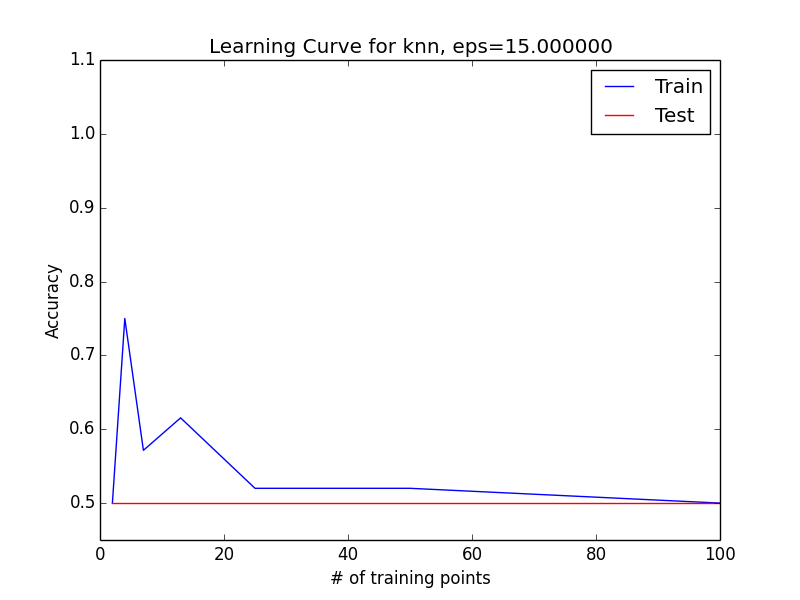
\includegraphics[scale = .45]{LC_eps15_000000.png}
		\end{subfigure}
		\hfill
		\begin{subfigure} [h!]{.4\textwidth}
		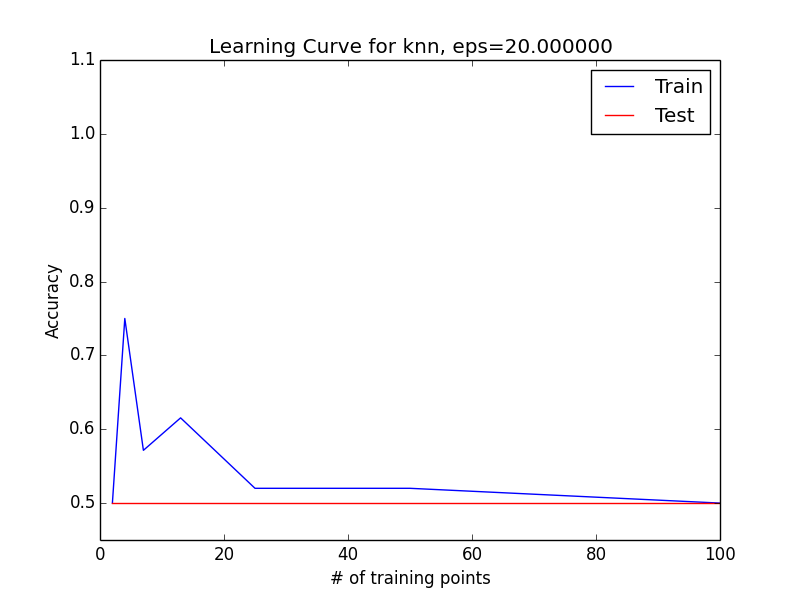
\includegraphics[scale = .45]{LC_eps20_000000.png}
		\end{subfigure}
		\caption{Learning curves for various $\epsilon$ values}
		\label{eps_figs}
	\end{figure}
	
	\clearpage
	
	\begin{figure} [h!]
		\centering
		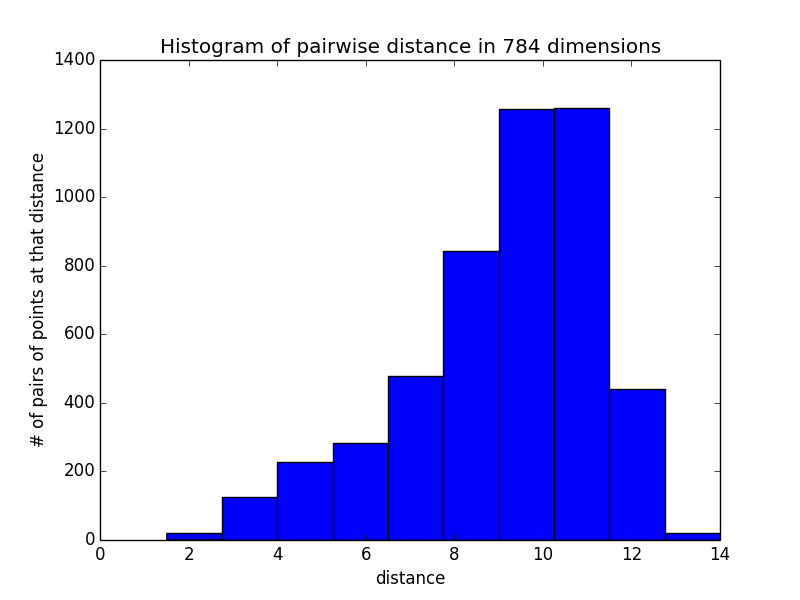
\includegraphics[scale = .65]{AllDims.png}
		\caption{Pairwise distances using all 784 dimensions}
		\label{alldims_fig}
	\end{figure}
		
	\begin{figure} [h!]
		\centering
		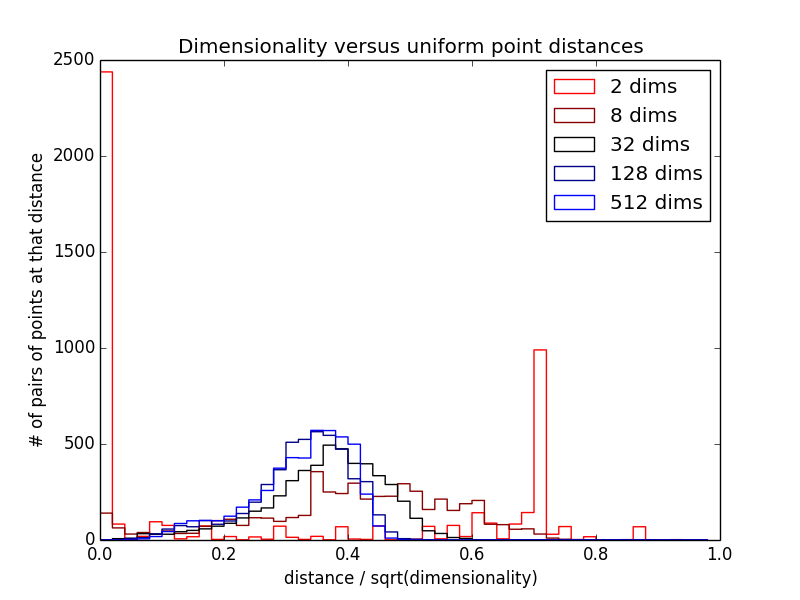
\includegraphics[scale = .65]{Subsampled.png}
		\caption{Pairwise distances using subsampled dimensions}
		\label{subsample_fig}
	\end{figure}
	
	\FloatBarrier
	
	\begin{figure} [h!]
		\centering
		
\includegraphics[scale = .65]{LC_perceptron.png}
		\caption{Learning curve for perceptron using 5 epochs}
		\label{lc_percept_fig}
	\end{figure}
		
	\begin{figure} [h!]
		\centering
		
\includegraphics[scale = .65]{Epochs_train_test.png}
		\caption{Effect of number of epochs on test/train accuracy}
		\label{epoch_tt_fig}
	\end{figure}
	
%	\begin{figure} [h!]
%		\begin{subfigure} [h!]{.4\textwidth}
%
%			\includegraphics[scale = .45]{initial_1485_400.png}
%			\caption{Initial data}
%			\captionsetup{justification=centering}
%		\end{subfigure}
%		\hfill
%		\begin{subfigure}[h!]{.4\textwidth}
%			
%			\includegraphics[scale = .45]{rk_stripe_raw_fig.png}
%			\caption{State at t=10}
%			\label{stripe_raw}
%			\captionsetup{justification=centering}
%		\end{subfigure}
%		\caption{Schakenberg simulation with $a=.05,$ $b=1.4,$ $e=14.85,$ $\gamma=400$}
%		\label{Stripe_figs}
%	\end{figure}
%	
%	\FloatBarrier	
	
	

	
\end{document}

